\begin{figure}[h!]
	\centering
	\begin{subfigure}[b]{0.3\textwidth}
		\centering
		\begin{adjustbox}{max width = \textwidth}
		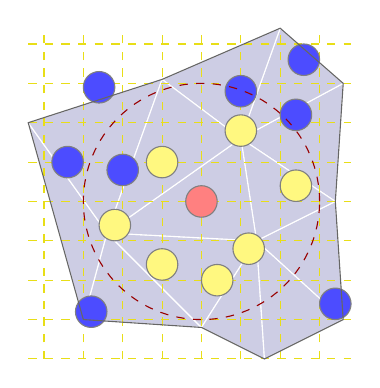
\begin{tikzpicture}
		%---Interno---
	%1 - (-1.2, -0.4)
	\draw[white, fill=blue!30!gray!30!white] (-1.5, -1.5) -- (0,-1.6) -- (-1.2, -0.4) -- cycle;
	\draw[white, fill=blue!30!gray!30!white] (-2.2, 1) -- (-1.5,-1.5) -- (-1.2, -0.4) -- cycle;
	\draw[white, fill=blue!30!gray!30!white] (-2.2, 1) -- (-0.5, 1.55) -- (-1.2, -0.4) -- cycle;
	%2 - (0.7, -0.5)
	\draw[white, fill=blue!30!gray!30!white] (-1.2, -0.4) -- (0,-1.6) -- (0.7, -0.5) -- cycle;
	\draw[white, fill=blue!30!gray!30!white] (0.8,-2) -- (0,-1.6) -- (0.7, -0.5) -- cycle;
	\draw[white, fill=blue!30!gray!30!white] (1.8,-1.5) -- (0.8,-2) -- (0.7, -0.5) -- cycle;
	\draw[white, fill=blue!30!gray!30!white] (1.8,-1.5) -- (1.7,0) -- (0.7, -0.5) -- cycle;
	%3 - (0.5,0.8)
	\draw[white, fill=blue!30!gray!30!white] (1.7,0) -- (1.8,1.5) -- (0.5, 0.8) -- cycle;
	\draw[white, fill=blue!30!gray!30!white] (1.7,0) -- (0.7, -0.5) -- (0.5, 0.8) -- cycle;
	\draw[white, fill=blue!30!gray!30!white] (1,2.2) -- (1.8,1.5) -- (0.5, 0.8) -- cycle;
	\draw[white, fill=blue!30!gray!30!white] (-0.5,1.55) -- (1,2.2) -- (0.5, 0.8) -- cycle;
	\draw[white, fill=blue!30!gray!30!white] (-1.2,-0.4) -- (0.7,-0.5) -- (0.5, 0.8) -- cycle;
	\draw[white, fill=blue!30!gray!30!white] (-1.2,-0.4) -- (-0.5,1.55) -- (0.5, 0.8) -- cycle;
	
	%malla
	\draw[step=0.5, dashed, yellow!90!black] (-2.2, -2) grid (1.9,2.2);
	
	%Partículas
	\draw[black!50, fill=red!50] (0,0) circle (2mm);
	\draw[black!50, fill=yellow!50] (0.6,-0.6) circle (2mm);
	\draw[black!50, fill=yellow!50] (-1.1,-0.3) circle (2mm);
	\draw[black!50, fill=yellow!50] (0.5,0.9) circle (2mm);
	\draw[black!50, fill=yellow!50] (-0.5,0.5) circle (2mm);
	\draw[black!50, fill=yellow!50] (1.2,0.2) circle (2mm);
	\draw[black!50, fill=yellow!50] (-0.5,-0.8) circle (2mm);
	\draw[black!50, fill=yellow!50] (0.2,-1) circle (2mm);
	
	\draw[black!50, fill=blue!70] (1.7,-1.3) circle (2mm);
	\draw[black!50, fill=blue!70] (-1.4,-1.4) circle (2mm);
	\draw[black!50, fill=blue!70] (-1,0.4) circle (2mm);
	\draw[black!50, fill=blue!70] (-1.7, 0.5) circle (2mm);
	\draw[black!50, fill=blue!70] (-1.3,1.45) circle (2mm);
	\draw[black!50, fill=blue!70] (1.2, 1.1) circle (2mm);
	\draw[black!50, fill=blue!70] (0.5,1.4) circle (2mm);
	\draw[black!50, fill=blue!70] (1.3,1.8) circle (2mm);
	
	%Carcasa
	\draw[black!60] (-2.2, 1) -- (-0.5, 1.55) -- (1, 2.2) -- (1.8, 1.5) -- (1.7, 0) -- (1.8, -1.5) -- (0.8, -2) -- (0, -1.6) -- (-1.5, -1.5) -- cycle;
	 
	 %Círculo rojo
	\draw[red!60!black, dashed] (0,0) circle (1.5 cm);
		\end{tikzpicture}
		\end{adjustbox}
		\caption{B\'usqueda de part\'iculas vecinas y c\'alculo de la fracci\'on de vac\'io de una part\'icula dada.}
	\end{subfigure}
	\hfill
	\begin{subfigure}[b]{0.3\textwidth}
		\centering
		\begin{adjustbox}{max width = \textwidth}
		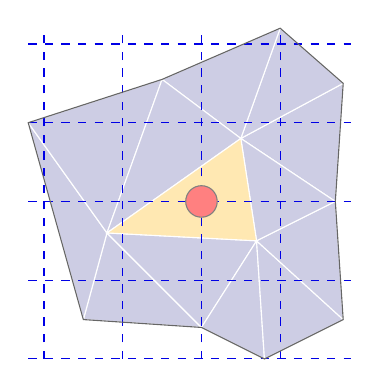
\begin{tikzpicture}
		%---Interno---
	%1 - (-1.2, -0.4)
	\draw[white, fill=blue!30!gray!30!white] (-1.5, -1.5) -- (0,-1.6) -- (-1.2, -0.4) -- cycle;
	\draw[white, fill=blue!30!gray!30!white] (-2.2, 1) -- (-1.5,-1.5) -- (-1.2, -0.4) -- cycle;
	\draw[white, fill=blue!30!gray!30!white] (-2.2, 1) -- (-0.5, 1.55) -- (-1.2, -0.4) -- cycle;
	%2 - (0.7, -0.5)
	\draw[white, fill=blue!30!gray!30!white] (-1.2, -0.4) -- (0,-1.6) -- (0.7, -0.5) -- cycle;
	\draw[white, fill=blue!30!gray!30!white] (0.8,-2) -- (0,-1.6) -- (0.7, -0.5) -- cycle;
	\draw[white, fill=blue!30!gray!30!white] (1.8,-1.5) -- (0.8,-2) -- (0.7, -0.5) -- cycle;
	\draw[white, fill=blue!30!gray!30!white] (1.8,-1.5) -- (1.7,0) -- (0.7, -0.5) -- cycle;
	%3 - (0.5,0.8)
	\draw[white, fill=blue!30!gray!30!white] (1.7,0) -- (1.8,1.5) -- (0.5, 0.8) -- cycle;
	\draw[white, fill=blue!30!gray!30!white] (1.7,0) -- (0.7, -0.5) -- (0.5, 0.8) -- cycle;
	\draw[white, fill=blue!30!gray!30!white] (1,2.2) -- (1.8,1.5) -- (0.5, 0.8) -- cycle;
	\draw[white, fill=blue!30!gray!30!white] (-0.5,1.55) -- (1,2.2) -- (0.5, 0.8) -- cycle;
	\draw[white, fill=blue!30!gray!30!white] (-1.2,-0.4) -- (-0.5,1.55) -- (0.5, 0.8) -- cycle;
	\draw[white, fill=red!30!yellow!30!white] (-1.2,-0.4) -- (0.7,-0.5) -- (0.5, 0.8) -- cycle;
	
	%malla
	\draw[step=1, dashed, blue!90!black] (-2.2, -2) grid (1.9,2.2);
	
	%Partículas
	\draw[black!50, fill=red!50] (0,0) circle (2mm);
	
	%Carcasa
	\draw[black!60] (-2.2, 1) -- (-0.5, 1.55) -- (1, 2.2) -- (1.8, 1.5) -- (1.7, 0) -- (1.8, -1.5) -- (0.8, -2) -- (0, -1.6) -- (-1.5, -1.5) -- cycle;
	 
		\end{tikzpicture}
		\end{adjustbox}
	\caption{Mapeo de una part\'icula dada dentro del fluido para interpolar sus propiedades en ese punto.}
	\end{subfigure}
	\hfill
	\begin{subfigure}[b]{0.3\textwidth}
		\centering
		\begin{adjustbox}{max width = \textwidth}
		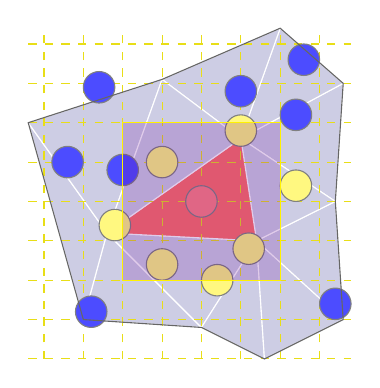
\begin{tikzpicture}
		%---Interno---
	%1 - (-1.2, -0.4)
	\draw[white, fill=blue!30!gray!30!white] (-1.5, -1.5) -- (0,-1.6) -- (-1.2, -0.4) -- cycle;
	\draw[white, fill=blue!30!gray!30!white] (-2.2, 1) -- (-1.5,-1.5) -- (-1.2, -0.4) -- cycle;
	\draw[white, fill=blue!30!gray!30!white] (-2.2, 1) -- (-0.5, 1.55) -- (-1.2, -0.4) -- cycle;
	%2 - (0.7, -0.5)
	\draw[white, fill=blue!30!gray!30!white] (-1.2, -0.4) -- (0,-1.6) -- (0.7, -0.5) -- cycle;
	\draw[white, fill=blue!30!gray!30!white] (0.8,-2) -- (0,-1.6) -- (0.7, -0.5) -- cycle;
	\draw[white, fill=blue!30!gray!30!white] (1.8,-1.5) -- (0.8,-2) -- (0.7, -0.5) -- cycle;
	\draw[white, fill=blue!30!gray!30!white] (1.8,-1.5) -- (1.7,0) -- (0.7, -0.5) -- cycle;
	%3 - (0.5,0.8)
	\draw[white, fill=blue!30!gray!30!white] (1.7,0) -- (1.8,1.5) -- (0.5, 0.8) -- cycle;
	\draw[white, fill=blue!30!gray!30!white] (1.7,0) -- (0.7, -0.5) -- (0.5, 0.8) -- cycle;
	\draw[white, fill=blue!30!gray!30!white] (1,2.2) -- (1.8,1.5) -- (0.5, 0.8) -- cycle;
	\draw[white, fill=blue!30!gray!30!white] (-0.5,1.55) -- (1,2.2) -- (0.5, 0.8) -- cycle;
	\draw[white, fill=red!95!yellow!60!white] (-1.2,-0.4) -- (0.7,-0.5) -- (0.5, 0.8) -- cycle;
	\draw[white, fill=blue!30!gray!30!white] (-1.2,-0.4) -- (-0.5,1.55) -- (0.5, 0.8) -- cycle;
	
	%malla
	\draw[step=0.5, dashed, yellow!90!black] (-2.2, -2) grid (1.9,2.2);
	
	%Partículas
	\draw[black!50, fill=red!50] (0,0) circle (2mm);
	\draw[black!50, fill=yellow!50] (0.6,-0.6) circle (2mm);
	\draw[black!50, fill=yellow!50] (-1.1,-0.3) circle (2mm);
	\draw[black!50, fill=yellow!50] (0.5,0.9) circle (2mm);
	\draw[black!50, fill=yellow!50] (-0.5,0.5) circle (2mm);
	\draw[black!50, fill=yellow!50] (1.2,0.2) circle (2mm);
	\draw[black!50, fill=yellow!50] (-0.5,-0.8) circle (2mm);
	\draw[black!50, fill=yellow!50] (0.2,-1) circle (2mm);
	
	\draw[black!50, fill=blue!70] (1.7,-1.3) circle (2mm);
	\draw[black!50, fill=blue!70] (-1.4,-1.4) circle (2mm);
	\draw[black!50, fill=blue!70] (-1,0.4) circle (2mm);
	\draw[black!50, fill=blue!70] (-1.7, 0.5) circle (2mm);
	\draw[black!50, fill=blue!70] (-1.3,1.45) circle (2mm);
	\draw[black!50, fill=blue!70] (1.2, 1.1) circle (2mm);
	\draw[black!50, fill=blue!70] (0.5,1.4) circle (2mm);
	\draw[black!50, fill=blue!70] (1.3,1.8) circle (2mm);
	
	%Carcasa
	\draw[black!60] (-2.2, 1) -- (-0.5, 1.55) -- (1, 2.2) -- (1.8, 1.5) -- (1.7, 0) -- (1.8, -1.5) -- (0.8, -2) -- (0, -1.6) -- (-1.5, -1.5) -- cycle;
	
	\draw[yellow, fill=red!40!blue, fill opacity=0.2] (-1,-1) rectangle (1,1);
		\end{tikzpicture}
		\end{adjustbox}
	\caption{Mapeo del elemento de malla CFD para el c\'alculo de t\'erminos fuente en el elemento de inter\'es.}
	\end{subfigure}
	\caption{Esquema de la aproximaci\'on por malla dual para la b\'usqueda de part\'iculas vecinas en un fluido.}
	\label{particle}
\end{figure}